\documentclass[12pt]{article}

\usepackage{times}
\usepackage{graphicx}
\usepackage{datetime}
\usepackage[utf8]{inputenc}
\usepackage[slovene]{babel}
\usepackage[font=]{caption}

\usepackage{listings}
\usepackage{color}
\usepackage{dirtree}

\definecolor{folderbg}{RGB}{124,166,198}
\definecolor{folderborder}{RGB}{110,144,169}

\definecolor{dkgreen}{rgb}{0,0.6,0}
\definecolor{gray}{rgb}{0.5,0.5,0.5}
\definecolor{mauve}{rgb}{0.58,0,0.82}
\definecolor{darkblue}{rgb}{0.0,0.0,0.6}

\lstset{
	basicstyle=\ttfamily,
	columns=fullflexible,
	showstringspaces=false,
	commentstyle=\color{gray}\upshape
}

\lstdefinelanguage{XML}
{
	morestring=[b]",
	morestring=[s]{>}{<},
	morecomment=[s]{<?}{?>},
	stringstyle=\color{black},
	identifierstyle=\color{darkblue},
	keywordstyle=\color{cyan},
	morekeywords={xmlns,version,type}
}

\lstdefinestyle{XmlStyle}{
	language=XML,
	aboveskip=3mm,
	belowskip=3mm,
	showstringspaces=false,
	columns=flexible,
	basicstyle={\small\ttfamily},
	numbers=none,
	keywordstyle=\color{blue},
	breaklines=true,
	tabsize=4
}

\lstdefinestyle{JavaStyle}{
	language=Java,
	aboveskip=3mm,
	belowskip=3mm,
	showstringspaces=false,
	columns=flexible,
	basicstyle={\small\ttfamily},
	numbers=none,
	numberstyle=\tiny\color{gray},
	keywordstyle=\color{blue},
	commentstyle=\color{dkgreen},
	stringstyle=\color{mauve},
	breaklines=true,
	tabsize=4
}

\newdateformat{MMYYYYdate}{\monthname[\THEMONTH] \THEYEAR}
\title{Riptide - Univerzalno orodje za konfiguracijo omrežij}
\author{Jurij Fortuna, G 3. a}
\date{\MMYYYYdate\today}

\begin{document}

\begin{center}
	\thispagestyle{empty}
	
\includegraphics[scale=1]{slike/vegova.png}

	\vspace{\fill}
	Seminarska naloga pri predmetu računalništvo

	\Huge{Riptide - Univerzalno orodje za konfiguracijo omrežij}

	\normalsize
	\vspace{\fill}

	Mentor: Marko Kastelic \hfill Avtor: Jurij Fortuna, G 3. a\\
	\null
	Ljubljana, \MMYYYYdate\today
\end{center}
\newpage

% Povzetek
\section*{Povzetek}
Naloga opisuje razvojni proces in delovanje programa Riptide. Riptide je
odprtokodna programska oprema, razvita v jeziku Java, namenjena
nastavitvi omrežnih naprav. Na začetku naloge je podan kratek pregled dveh
glavnih komponent programske opreme: osprednega dela in aplikacijskega
programskega vmesnika (API). V nadaljevanju dokument opisuje ''Shede'',
vtičnike za komunikacijo z omrežno opremo. Naloga se zaključi s primerom
razvoja Sheda in obravnava izzive, povezane z njim.
\\\\
\textbf{Ključe besede:} omrežja, omrežne naprave, nastavitev omrežij, API,
odprtokodna programska oprema
\\
\section*{Abstract}
\foreignlanguage{english}{
	The purpose of this paper is to report on the development process and
	inner workings of Riptide. Riptide is an open-source software developed
	in Java for configuring network devices. It addresses the issue of
	using multiple software solutions from different manufacturers to
	configure networks. Initially, the document gives a brief overview of
	two main components of the software: the frontend and the Application
	Programming Interface (API). Following that, the document describes
	''Sheds,'' plugins for interacting with network equipment. The paper
	concludes by documenting the development of a custom Shed and discusses
	the associated challenges that can arise during the development.
	\\\\
	\textbf{Keywords:} networking, network devices, network setup, API,
	open-source software
}
\newpage

% Kazalo
\tableofcontents
\newpage

% 1. Uvod
\section{Uvod}
Ideja za razvoj Riptide-a se je pojavila, ko sem bil med konfiguracijo
domačega omrežja prisiljen uporabljati tri vrste programske opreme,
različnih proizvajalcev. Med sabo so se nemalo razlikovale in so bile
po večini nestabilne. Rezultat naloge je programska oprema Riptide.
Deluje na principu “vtičnikov” (t.i. Shedov) za posamezne kose omrežne
opreme, kar uporabnikom omogoča, da iz enega programa nastavljajo celotno
svoje omrežje. Programska oprema je odprtokodna in brezplačna, kar omogoča
večjo dostopnost uporabnikom.
\\\\

\begin{center}
	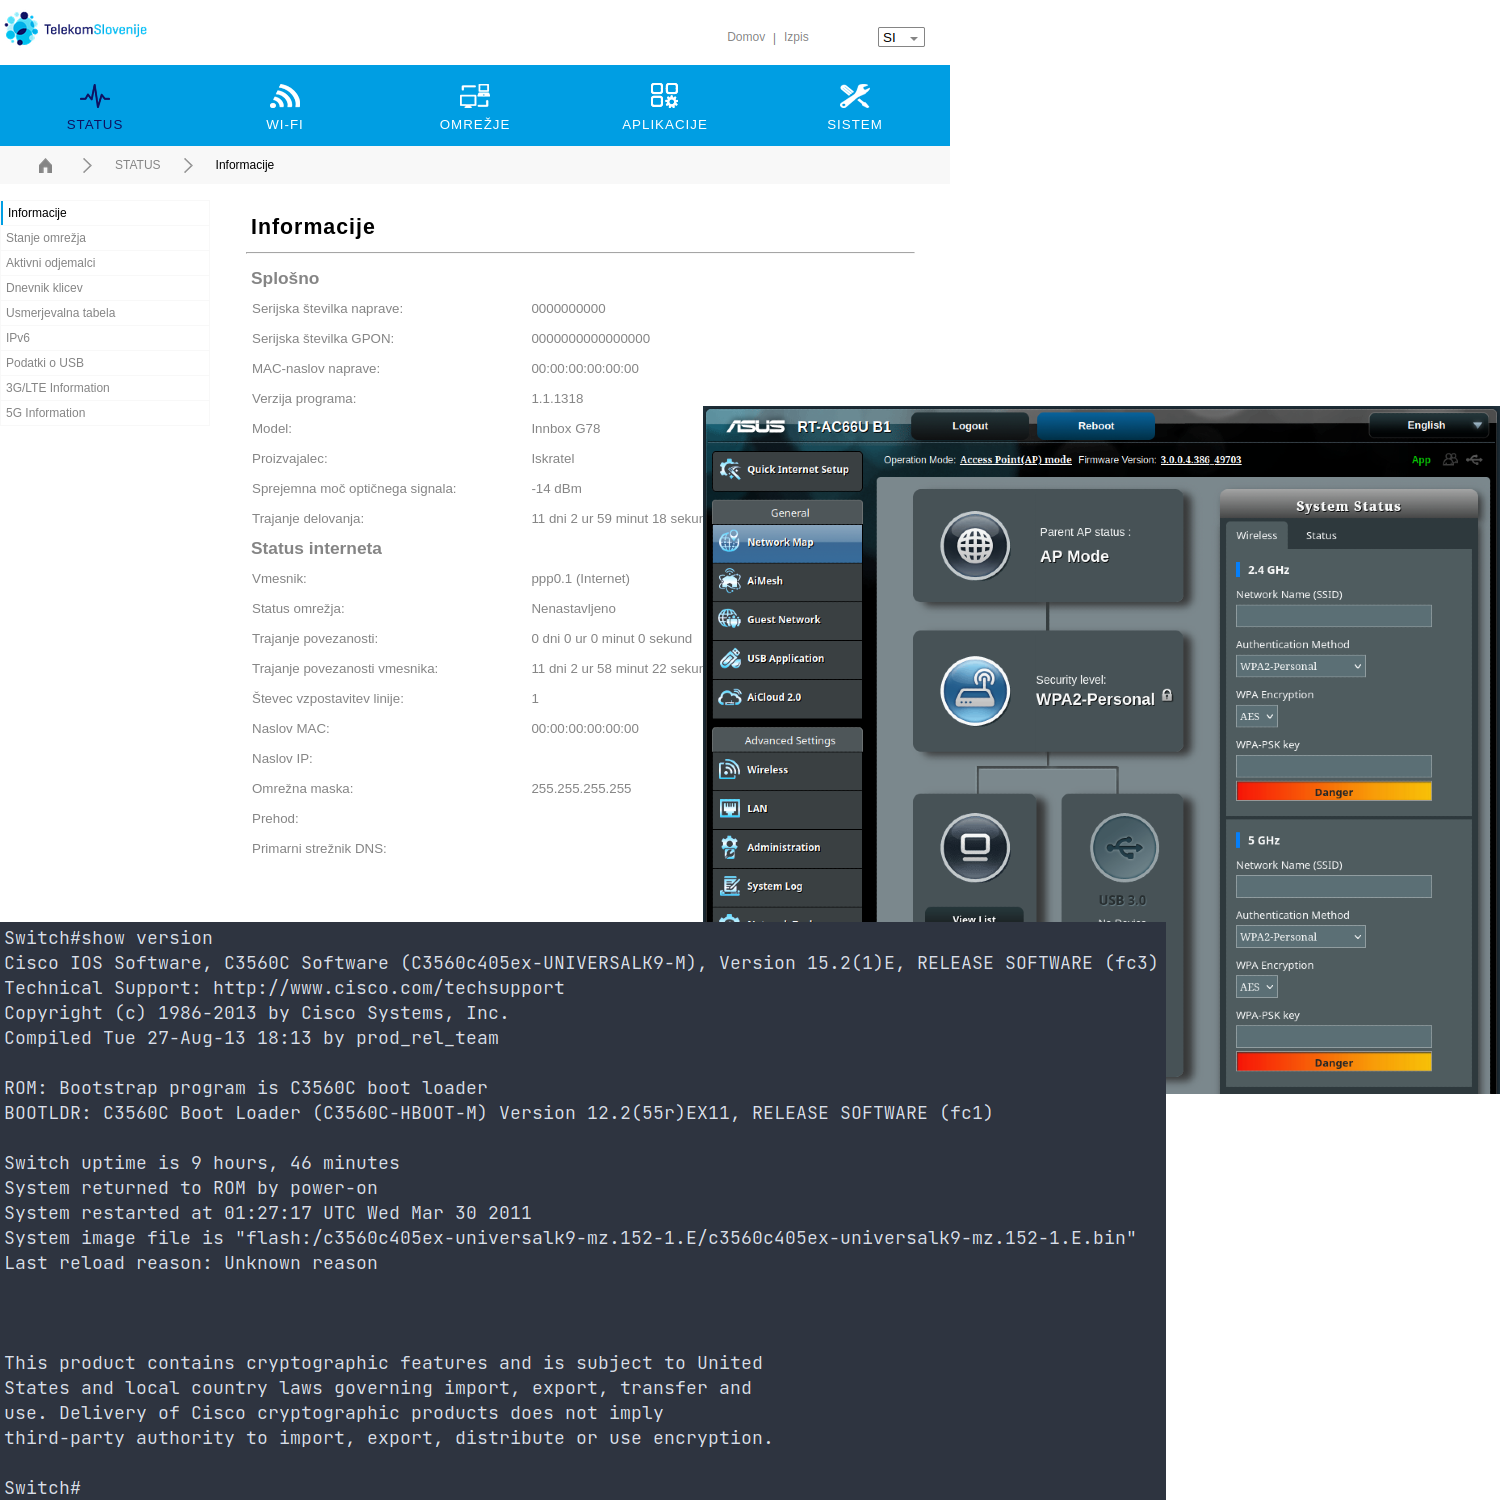
\includegraphics[scale=0.24]{slike/config.png}
	\captionof{figure}{Primeri uporabljene programske opreme}
\end{center}
\newpage

% 2. Tehnologije
\section{Uporabljene tehnologije}
Tako Shedi, kot tudi Riptide so napisani v Javi. Java omogoča dinamično
nalaganje modulov ob zagonu navideznega stroja, tudi iz zapakiranih JAR
datotek. Aplikacijo sestavljajo trije deli: Ospredni del, API in Shedi. Med
sabo so to ločeni deli in razvoj poteka na vsakem posamezno. V nadaljevanju
naloge bo vsak podrobneje opisan.

\subsection{Ospredni del}
Ospredni del je del, s katerim uporabnik upravlja. Skrbi za prikaz podatkov
in vnašanje konfiguracije. Skrbi tudi za shranjevanje poverlinic in
upravljanje z uporabnikovimi podatki.

\subsection{Aplikacijski programski vmesnik}
Aplikacijski programski vmesnik (v nadaljevanju API) deluje kot most med
osprednim delom in Shedi. Z njim lahko preko vmesnikov ospredni del ukaze
pošilja Shedom.

\subsection{Shedi}
Shedi so vtičniki, oziroma gonilniki, ki skrbijo za komunikacijo z 
omrežnimi napravami. Razviti so s pomočjo Riptide SDK-ja in praviloma
odprtokodni.

\begin{center}
	
\includegraphics[scale=0.5]{slike/zgradba.png}
	\captionof{figure}{Diagram delovanja}
\end{center}
\newpage

% 3. Ospredni del
\section{Ospredni del}
Ospredni del je odgovoren za konfiguracijo Riptide-a ter rokovanje z 
uporabnikovimi poverilnicami in napravami.

\subsection{Uporabniški vmesnik}
Za izgradnjo uporabniškega vmesnika sem uporabil knjižnico JavaFX. Omogoča
hitro izdelavo in načrtovanje, skupaj s knjižnico FXML. Za stil pa sem
uporabil knjižnico AtlantaFX, ki naredi vmesnik minimalističen in vključuje
štiri že narejene stilske datoteke.
\\\\
Glavno okno za konfiguracijo naprav je zasnovano kot MDI (ang.
multiple-document interface). Glavna prednost MDI-ja je možnost rabe večih
podoken znotraj glavnega okna, kar uporabniku omogoča večopravilnost.

\subsection{Konfiguracija}
Uporabnik lahko svoje naprave shrani, in si s tem prihrani čas za
morebitno kasnejšo konfiguracijo. Poleg tega Riptide omogoča spremembo
barve vmesnika po uporabnikovi želji.
\\\\
Okoljske spremenljivke, naprave in poverilnice so zapisanje v objektu
imenovanem \texttt{Workspace}.

\begin{lstlisting}[style=JavaStyle]
@Data
public class Workspace implements Serializable {
	private Theme theme;
	private ArrayList<Credential> credentials;
	private ArrayList<Connection> connections;

	public Workspace() {
		theme = Theme.PRIMER_DARK;
		credentials = new ArrayList<>();
		connections = new ArrayList<>();
	}

	public Workspace(Theme theme, ArrayList<Credential> credentials, ArrayList<Connection> connections) {
		this.theme = theme;
		this.credentials = credentials;
		this.connections = connections;
	}
}
\end{lstlisting}
Ko uporabnik nastavitve shrani je objekt serializiran in zapisan v datoteko
na uproabnikov sistem. Datotek je lahko več, kar omogoča prilagoditev
vmesnika za različna okolja (npr. posebej za domačo in poslovno rabo).
Workspace datoteke so shranjene v JSON formatu, kar uporabnikom omogoča
enostavno izmenjavo ali prenos.

\subsection{Upravljanje poverilnic}
Za konfiguracijo večine omrežnih naprav je potrebna avtorizacija.
Riptide uporabnikom omogoča varno shranjevanje poverilnic na njihovem
sistemskem keyringu. Poverilnice so ob povezavi na napravo prek API-ja
podani Shedu, kar pomeni, da se razvijalci teh ne rabijo ukvarjati z
varnim hranjenjem poverilnic.

\subsection{Rokovanje z napravami}
\subsubsection{Nalaganje Shedov} \label{nalaganje-shedov}
Nalaganje shedov poteka v dveh korakih, lociranje Sheda in branje
metapodatkov. Na uporabnikovem sistemu se nahajajo v obliki JAR datotek v
dveh mapah, \texttt{\textasciitilde/.config/Riptide/sheds} na *NIX sistemih
in \texttt{\%UserProfile\%\textbackslash\\.Riptide\textbackslash sheds} na
Windows sistemih.

\subsubsection{Nalaganje naprav} \label{nalaganje-naprav}
Ob izbiri naprave, Riptide iz Shedovih metapodatkov najprej prebere
njen t.i. model path, ki izgleda približno
tako: \texttt{telekomslovenije.innboxg78.ts}. Niz je sestavljen iz ID-ja
Sheda, ID-ja modela nprave in ID-ja različice modela. Vsi ID-ji so
edinstveni, kar pomeni, da lahko program najde Shed, v njem poišče model
naprave, njegovo različico in vzpostavi povezavo z napravo prek API-ja.
\newpage

% 4. Aplikacijski programski vmesnik
\section{Aplikacijski programski vmesnik}
API omogoča uporabnikom, da ustvarijo lastno podporo za omrežno
opremo, ki je programska oprema še ne podpira. To pomeni, da lahko
skrbniki omrežij enostavno integrirajo nove naprave v svoje omrežje, ne da
bi morali čakati, da prodajalec izda uradno podporo.

\subsection{Dostop do API-ja}
Dostop do APIja je mogoč preko SDK knjižnice. Nahaja se v Riptide
Maven repozitoriju. Ker so Javanski upravitelji paketov med seboj bolj
kot ne kompatibilni, je tudi postopek dodajanja knjižnice med njimi
zelo podoben. Več o strukturi projekta pa v razdelku
\ref{struktura-projekta}.

\subsection{Struktura API-ja}
Vsi pomembni vmesniki in razredi za pisanje Shedov se nahajajo v
paketu \texttt{org\-.riptide.sdk.sheds}. Paket je deljen na podpakete za
uporabniški vmesnik, tipe naprav, čarovnike in avtentikacijo.

\subsection{Vgrajena orodja}
API vsebuje uporabna orodja za izdelovanje statusnih strani in
formularjev, ki se nahajajo v paketu \texttt{org.riptide.sdk.sheds.ui}.

\subsection{Komunikacija z napravami} \label{komunikacija-z-napravami}
Ospredni del s Shedi komunicira preko vmesnikov. Za primer vzemimo
Telekomov usmerjevalnik. Ob izbiri naprave se instancira njen gonilni
razred v nov objekt, ki je odgovoren za komunikacijo z napravo
(postopek je opisan v razdelku \ref{nalaganje-naprav}).
\\\\
Program iz metapodatkov razbere, da naprava tipa router. To pomeni,
da mora njen gonilni razred implementirati vmesnik \texttt{Router} in
posledično \texttt{Device}, saj ga \texttt{Router} razširja.
\newpage

\begin{lstlisting}[style=JavaStyle]
public interface Device {
	void initialize(String address, Credential credential);
	LinkedHashMap<String, Tab[]> getPages();
}

public interface Router extends Device {
	PATWizard patWizard();
}
\end{lstlisting}
Za tem se kliče metoda \texttt{initialize/2}, ki gonilnemu objektu poda
omrežni naslov naprave in poverilnice.
\\\\
Nato program od gonilnega objekta zahteva seznam konfiguracijskih strani
in zavihke z metodo \texttt{getPages/0} (glej \ref{konfiguracijske-strani}).
Ospredni del jih z orodnim razredom \texttt{ContentRenderer} generira, tako
kot primer spodaj.

\begin{center}
	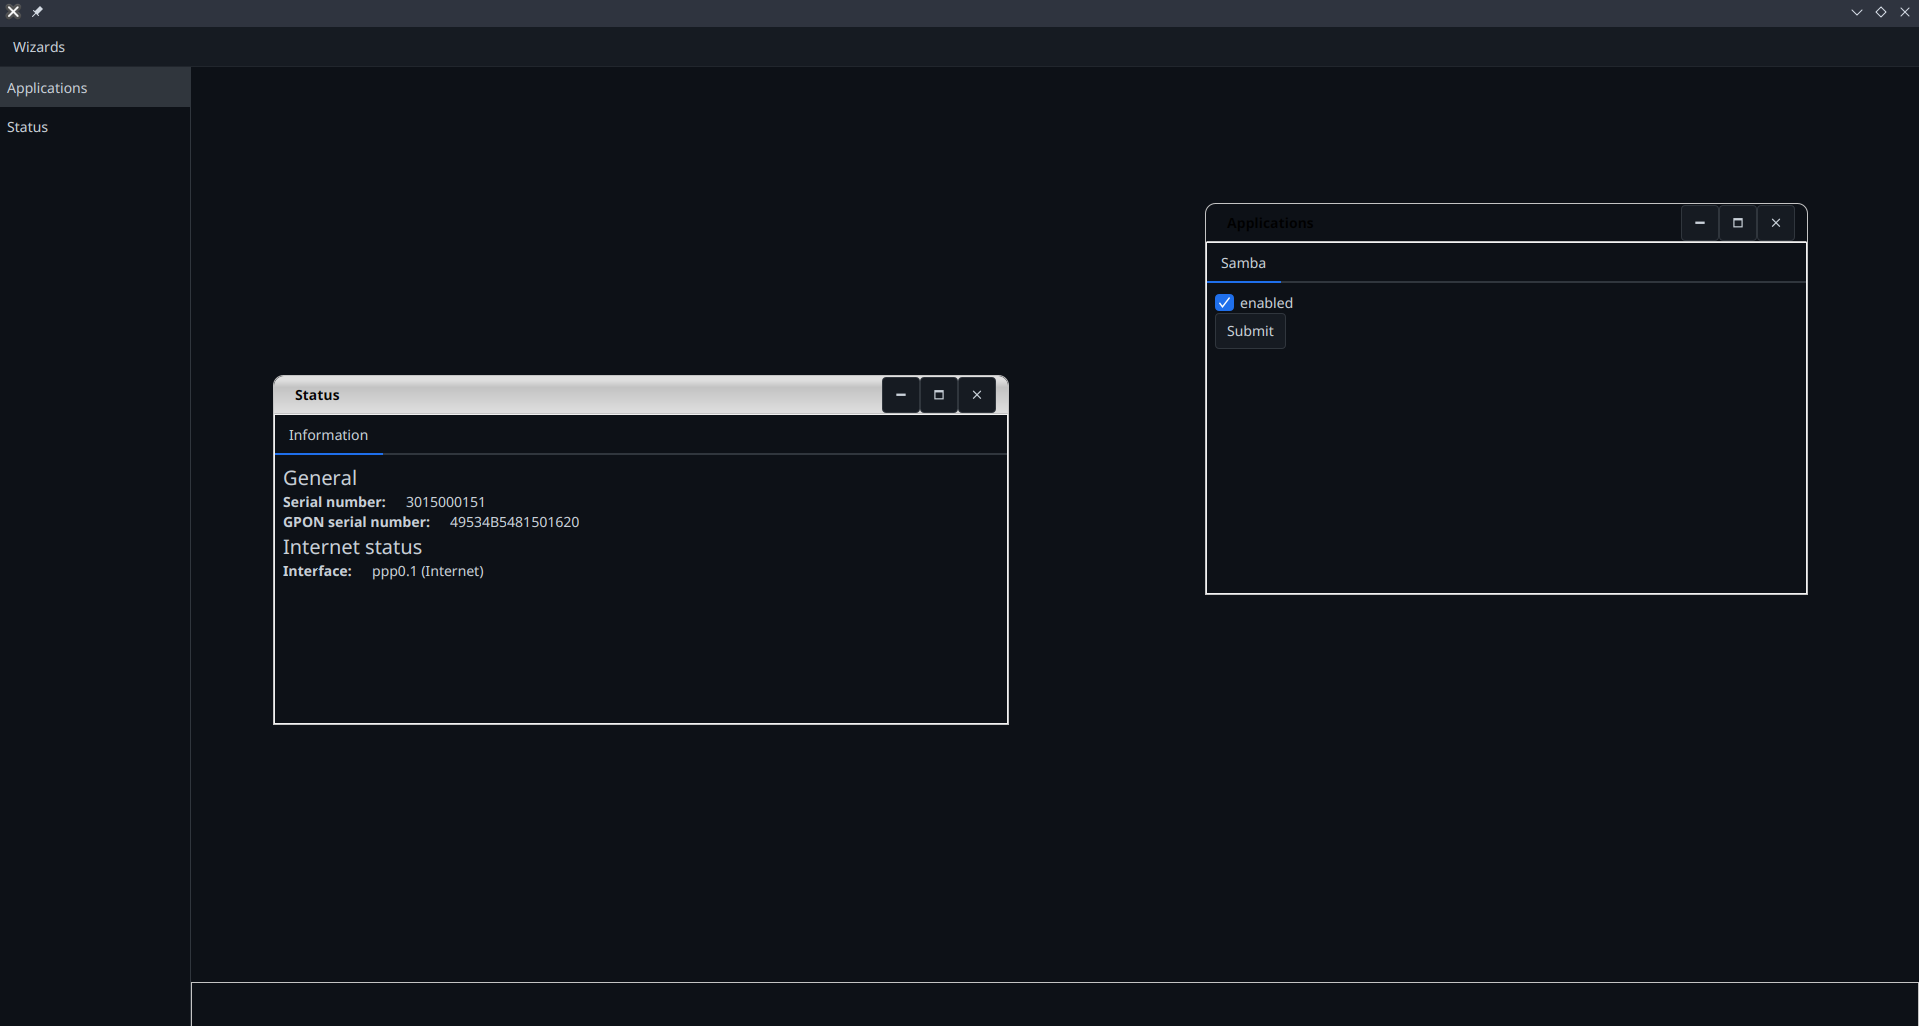
\includegraphics[scale=0.28]{slike/config-window.png}
	\captionof{figure}{Primer generirane konfiguracijske strani}
\end{center}
\newpage

\subsection{Čarovniki}
Program tudi manj naprednim uporabnikom omogoča nastavitev njihove omrežne
opreme. V glavnem oknu katerokoli omrežne naprave se v menijski vrstici
nahaja gumb ''Wizards''. Pod njem se glede na tip naprave pojavijo različne
podmožnosti. Za usmerjevalnike je to zaenkrat \textit{Port forwaring wizard},
ki omogoča uporabniku konfiguracijo NAT-a, za stikala pa
\textit{VLAN wizard}, ki omogoča konfiguracijo VLAN-ov.

\begin{center}
	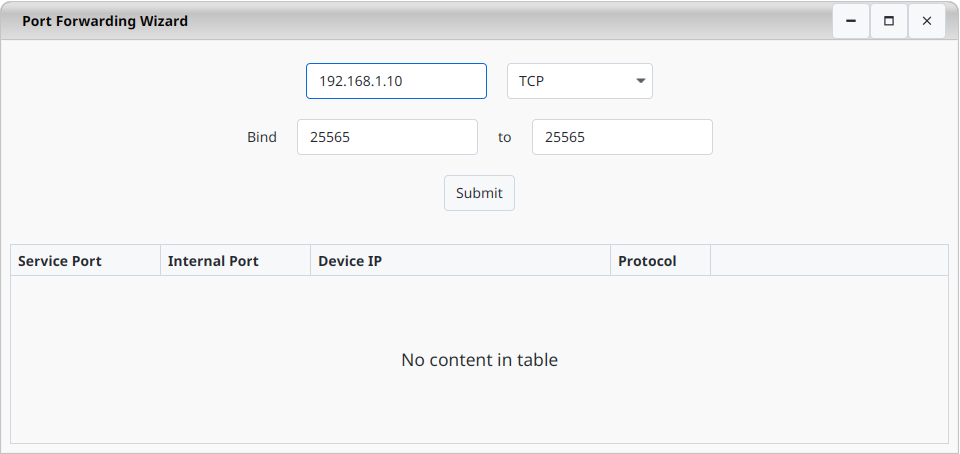
\includegraphics[scale=0.56]{slike/pat-wizard.png}
	\captionof{figure}{Čarovnik za konfiguracijo NAT-a}
\end{center}
\newpage

% 5. Shedi
\section{Shedi}
Shedi so vtičniki, ki skrbijo za komunikacijo z napravami. Sami po sebi
niso izvršljivi programi, vendar so le zbirka razredov. Zapakirani so v
JAR datoteke, skupaj z datoteko \texttt{shed.yml}.
\\\\
V prihodnosti načrtujem omogočiti razširitev tudi drugih funkcionalnosti.
Zaradi tega sem se za poimenovanje vtičnikov naprav odločil uporabiti
izraz ''shedi'' namesto običajnega izraza ''plugin''.

\subsection{Priprava projekta}
Pri pripravi projekta je bil uporabljen standardni javanski upravitelj
paketov \textit{Apache Maven}. Za začetek je potrebno dodati repozitorij in
knjižnico. To naredimo v datoteki \texttt{pom.xml}.

\begin{lstlisting}[style=XmlStyle]
<repositories>
	<repository>
		<id>repsy</id>
		<url>https://repo.repsy.io/mvn/riptide/maven</url>
	</repository>
</repositories>

<dependencies>
	<dependency>
		<groupId>org.riptide</groupId>
		<artifactId>sdk</artifactId>
		<version>VERZIJA</version>
	</dependency>
</dependencies>
\end{lstlisting}
\newpage

\subsection{Struktura projekta} \label{struktura-projekta}
\begin{dirtree}{%
.1 NasShed.
	.2 src.
		.3 main.
			.4 java.
				.5 organizacija.
					.6 artefakt.
						.7 GonilniRazred.java.
			.4 resources.
				.5 shed.xml.
	.2 pom.xml.
}
\end{dirtree}
\vspace*{12pt}
V privzeti paket (oziroma podpakete) dodamo gonilne razrede za naše naprave.
V \texttt{resources} mapo pa datoteko \texttt{shed.yml}, ki bo vsebovala
metapodatke o Shedu.

\subsubsection{Metapodatki}
Metapodatki vsebujejo pomembne informacije o Shedu. Med drugimi vključujejo
unikatne identifikatorje, ki so nujni za delovanje. Metapodatki so
shranjeni v datoteki \texttt{shed.yml}.

\begin{lstlisting}[style=XmlStyle]
name: "Telekom Slovenije Shed"
id: "telekomslovenije"
version: "1.0"
api_level: "1.0"
authors:
	- "chocoearly44"
routers:
	- name: "InnboxG78"
	id: "innboxg78"
	flavours:
		- name: "Telekom Slovenije"
		id: "ts"
		handler: "org.riptide.ts.Main"
switches:
\end{lstlisting}
Zaglavje vsebuje ime Sheda, njegov ID, verzijo, avtorje in podprto verzijo
API-ja, za katero je bil zgrajen. Pod zaglavjem sledijo razdelki s tipi
naprav. V njih so shranjene podprte naprave, ki vsebujejo imena, ID-je in
vrste. Vrste (flavours) vsebujejo poti do gonilnih razredov, saj ima naprava
lahko različne funkcionalnosti, glede na nameščeno programsko opremo. Tako
zagotovimo, da lahko isti Shed podpira isto napravo, ne glede na
distributerja (za primer InnboxG78 usmerjevalnik, katerega distribuirata
tako Telekom Slovenije, kot tudi T2).

\subsubsection{Gonilni razredi}
Gonilni razredi komunicirajo z napravami. Za pravilno delovanje, morajo
implementirati enega izmed v naprej narejenih vmesnikov (npr.
\texttt{Router} ali \texttt{Switch}), zaradi dedovanja pa posledično
implementirajo tudi \texttt{Device} vmesnik. V njih so definirane metode
za inicializacijo povezave, ipd. Postopek vzpostavitve povezave pa je
opisan v razdelku \ref{komunikacija-z-napravami}.

\subsubsection{Konfiguracijske strani} \label{konfiguracijske-strani}
Konfiguracijske strani so strani v podoknu, kjer so zbrane nastavitve
naprave, ločenih z zavihki. V Shedu so predstavljene z razredi, ki
implementirajo \texttt{Tab} vmesnik.

\begin{lstlisting}[style=JavaStyle]
public interface Tab {
	String getTitle();
	UIComponent rootComponent();
}
\end{lstlisting}
Metoda \texttt{getTitle/0} vrača naslov zavihka, metoda
\texttt{rootComponent/0} pa komponento uporabniškega vmesnika, ki se bo
pokazala v zavihku (npr. tabela, kontejner, formular, ...).
\\\\
Objekti teh zavihkov so nato zbrani v tabelo, katera se preslika v niz s
pomočjo razreda \texttt{LinkedHashMap}. Taka preslikava bo predstavljala
konfiguracijko stran, ki jo lahko odpremo iz stranske vrstice. Te
preslikave nato zberemo in jih vrnemo v metodi \texttt{getPages/0}.

\subsection{Izgradnja}
Zadnji korak razvoja Sheda je izgradnja. Ko projekt gradimo, moramo paziti,
da v končno JAR datoteko vključimo morebitne knjižnice, ki smo jih
uporabili (npr. za komunikacijo preko SSH-ja). Izgrajeno JAR datoteko nato
uporabniki naložijo v mapo kjer imajo shranjene svoje Shede
(glej \ref{nalaganje-shedov}).
\newpage

% 6. Eksperimentalne funkcije
\section{Eksperimentalne funkcije}
Riptide je opremljen z nekaj novimi, eksperimentalnimi funkcijami, ki pa
jih zaradi pomanjkanja časa nisem uspel povsem dokončati in stestirati. Te
omogočajo naprednim uporabnikom nove možnosti avtomacije in pregleda nad
omrežjem.

\subsection{Topološki pogled omrežja}
Ta funkcionalnost omogoča pogled fizične topologije omrežja, podoben, kot
pri Ciscovem Packet Tracerju. Prikazane naprave lahko uporabniki povežejo
med sabo oziroma jih dvokliknejo za hitrejšo konfiguracijo.

\subsection{Integracija z Luo}
Riptide ima vgrajeno Lua izvajalno okolje. Lua je preprost programski jezik,
s katerim lahko administratorji pišejo skripte. Te skripte omogočajo
avtomatizacijo konfiguracije omrežja in s tem prihranijo čas uporabnikom.
\newpage

% 7. Zaključek
\section{Zaključek}
Dobljeni rezultat predstavlja enostavno in stabilno rešitev za nastavitev
omrežij. Z rabo ''vtičnikov'' (Shedov) omogoča uporabnikom konfiguracijo
različne omrežne opreme na enostaven način.
\\\\
Z uporabo Riptide-a lahko skrbiki omrežij enostavno integrirajo nove
naprave v svoje omrežje, ne da bi morali čakati na uradno podporo
proizvajalca. S svojim aplikacijskim programskim vmesnikom (API) omogoča
razvijalcem ustvarjanje lastne podpore za omrežno opremo, ki je programska
oprema še ne podpira.
\newpage

% 8. Viri in literatura
\section{Viri in literatura}
lua. \textit{Lua: about}, 2023, spletni naslov: https://www.lua.org/about
.html (26. 5. 2023)
\\\\
mkpaz. \textit{AtlantaFX Overview}, 2023, spletni naslov: https://mkpaz.
github.io/atlantafx (31. 12. 2022)
\\\\
OpenJFX. \textit{Getting Started with JavaFX}, spletni naslov: https://
openjfx.io/openjfx-docs (31. 12. 2022)
\\\\
Oracle. \textit{URLClassLoader (Java SE 20 \& JDK 20)}, 2023, spletni
naslov: https://docs.oracle.com/en/java/javase/20/docs/api/java.base/java/
net/URLClassLoader.html (3. 3. 2023)
\newpage

\begin{samepage}
	\thispagestyle{empty}
	\section*{Priloge}
	\textbf{Priloga 1}\\
	Koda za ospredni del: https://github.com/riptideconfig/Riptide
	\\\\
	\textbf{Priloga 2}\\
	Koda za SDK: https://github.com/riptideconfig/SDK
	\\\\
	\textbf{Priloga 3}\\
	Koda za Shed Telekoma Slovenije: https://github.com/riptideconfig/TelekomShed
\end{samepage}
\newpage

% Izjava o avtorstvu
\begin{samepage}
	\thispagestyle{empty}
	\section*{Izjava o avtorstvu}
	Izjavljam, da je seminarska naloga v celoti moje avtorsko delo, ki sem
	ga izdelal samostojno s pomočjo navedene literature in pod vodstvom
	mentorja.
	\\\\
	\MMYYYYdate\today \hfill Jurij Fortuna
\end{samepage}

\end{document}